% PLEASE USE THIS FILE AS A TEMPLATE
% Check file iosart2x.tex for more examples

% add. options: [seceqn,secthm,crcready,onecolumn]
\documentclass[sw]{iosart2x}

%\usepackage{dcolumn}
%\usepackage{endnotes}

%para el simbolo de chequeado
\usepackage{amssymb}% http://ctan.org/pkg/amssymb
\usepackage{pifont}% http://ctan.org/pkg/pifont
\newcommand{\cmark}{\ding{51}}%
\newcommand{\xmark}{\ding{55}}%

%%%%%%%%%%% Put your definitions here
\newtheorem{example}{Example}

%%%%%%%%%%% End of definitions

\pubyear{0000}
\volume{0}
\firstpage{1}
\lastpage{1}

\begin{document}

\begin{frontmatter}

%\pretitle{}
\title{Dynamic Linked Open Data: A Survey}
\runningtitle{Dynamics on Linked Open Data: A Survey}
%\subtitle{}

% For one author:
%\author{\inits{N.}\fnms{Name1} \snm{Surname1}\ead[label=e1]{first@somewhere.com}}
%\address{Department first, \orgname{University or Company name},
%Abbreviate US states, \cny{Country}\printead[presep={\\}]{e1}}
%\runningauthor{N. Surname1}

% Two or more authors:
\author[A]{\inits{N.}\fnms{Alberto} \snm{Moya Loustaunau}\ead[label=e1]{amoya@dcc.uchile.cl}},
\author[A]{\inits{N.N.}\fnms{Aidan} \snm{Hogan}\ead[label=e2]{ahogan@dcc.uchile.cl}}
and
\author[B]{\inits{N.-N.}\fnms{Name} \snm{Surname}\ead[label=e3]{third@somewhere.com}}
\runningauthor{N. Surname1 et al.}
\address[A]{IMFD Chile; Department of Computer Science, \orgname{University of Chile}, \cny{Chile}\printead[presep={\\}]{e1,e2}}
\address[B]{Department first, \orgname{University or Company name},
Abbreviate US states, \cny{Country}\printead[presep={\\}]{e3}}

%\begin{review}{editor}
%\reviewer{\fnms{First} \snm{Editor}\address{\orgname{University or Company name}, \cny{Country}}}
%\reviewer{\fnms{Second} \snm{Editor}\address{\orgname{First University or Company name}, \cny{Country}
%    and \orgname{Second University or Company name}, \cny{Country}}}
%\end{review}
%\begin{review}{solicited}
%\reviewer{\fnms{First} \snm{Solicited reviewer}\address{\orgname{University or Company name}, \cny{Country}}}
%\reviewer{\snm{anonymous reviewer}}
%\end{review}
%\begin{review}{open}
%\reviewer{\fnms{First} \snm{Open Reviewer}\address{\orgname{University or Company name}, \cny{Country}}}
%\end{review}

\begin{abstract}
Linked Open Datasets contain descriptions that change over time. The resources described by these datasets are continuously created, moved, deleted, linked, and unlinked. Applications that leverage Linked Data must be aware of these change dynamics to deliver accurate services. Understanding and being able to deal with dynamic datasets is essential for delivering accurate responses. This has been acknowledged by researchers who responded by suggesting techniques for dealing with Data Dynamics. Despite its importance and the efforts of researchers, the current understanding of change dynamics for Linked Data is still incomplete. Our contribution is a systematic literature review on Dynamic Linked Open Data and gives an overview of the current approaches to detect, propagate, and describe changes in resources and datasets of the Linked Open Data Web, as well as, the approaches proposed to deal with them, identifying respective potentials and limits.
\end{abstract}

\begin{keyword}
\kwd{Data dynamics}
\kwd{Synchronization}
\kwd{Linked Open Data}
\end{keyword}

\end{frontmatter}

%%%%%%%%%%% The article body starts:

\section{Introduction}\label{Introduction}

The Semantic Web (SW) is an extension of the WWW towards a Web of Data (WD), where data on the Web are published through W3C\footnote{World Wide Web Consortium: https://www.w3.org/ } standards. The goal is to enable computers to do more automated tasks by developing systems that can support trusted interactions over the network. The Linked Data (LD) term points to a set of steps to distribute and connect structured data on the Web using SW standards. The LD principles\footnote{LD principles: https://www.w3.org/DesignIssues/LinkedData.html} provide a flexible publishing paradigm to integrate and interlink any kind of data from arbitrary datasets published by various data providers on the Web. Once LD is presented under an open license, it is called Linked Open Data (LOD). LD is empowered by the SW formats and technologies that enable it, such as RDF\footnote{Resource Description Framework: https://www.w3.org/RDF/} and SPARQL\footnote{Semantic Query Language: https://www.w3.org/TR/sparql11-overview/}, standardized approaches to create data stores and query them.

From the time that the LD principles have been created until now, Linked Data has grown significantly in the number of RDF datasets and the size of those datasets~\cite{SchmachtenbergBP14}. Additionally, a wide variety of applications use information sourced from the Web to offer services. Also, recent investigations~\cite{KaferAUOH13, UmbrichHHPD10, DividinoSGG13, AuerDML12, SchmachtenbergBP14} have shown that the data published and interlinked on the Web is subject to frequent changes. The volume and velocity of changes constitute important challenges that applications must handle to keep results up-to-date.

The distributed Web-based nature of the data requires LOD applications to keep local copies of the data in a cache for faster access at runtime. As the data on the Web changes, these caches or indexes no longer reflect the current state of the data anymore and need to be updated, but this is a major challenge, because the remote sources are updated autonomously and independently of the local copies.

Many works have tried to handle these challenges. On the one hand, the evolution of LOD datasets has been studied to understand and identify patterns that allow estimating future changes. On the other hand, techniques have been developed that allow applications to locally store the relevant data and to estimate the appropriate time to update them.

Umbrich et al.~\cite{UmbrichVH10} presented an overview of existing approaches to detect, propagate and describe changes in resources and the Linked Open Data Web. They also presented four use cases that require technical solutions to deal with dynamic data and provided an overview of their requirements. However, from the development of this work to the present, many works have been developed to these and new use cases, as well as, new technical solution have been proposed.

Today, as people develop increasingly sophisticated applications that exploit the very nature of the linked data, the robustness of the support infrastructure becomes increasingly important. Dataset dynamics affect application performance

Despite its importance, the current understanding of change dynamics for the data web is not enough. Thats why we perform a this Systematic Literature Reviews to summarise the existing evidence concerning a data dynamics in the Linked Open Data Web, to identify any gaps in current research in order to suggest areas for further investigation and to provide a framework/background in order to appropriately position new research activities.

\subsection{Survey Scopes}\label{Scopes}

This survey provides an overview of published works that directly involve with data dynamics on the Linked Open Data, as well as, the Aplications methods to deal with them, such as, detection, propagation, description, preservation and explotation.

Then, we show a list of use cases that could benefit from an understanding of the dynamics of the data on the data web and can have a potential impact on several use cases:


SandersonS12:synchronization, smart caching, link maintenance, and vocabulary evolution

UmbrichVH10:
3.1 Use Cases UC 1: Synchronisation
A dataset consumer wants to mirror or replicate (parts of) a dataset from the LOD cloud. Ideally, the consumer wants to be informed about the statements that have been added/removed at a certain time point. The notification about the changes enables him an efficient way to keep his dataset up-to-date. Most commonly, the synchronisation is either for a single data source or for a set of data sources.

3.2 Use Cases UC 2: Smart Caching A developer uses one or more datasets from the LOD cloud in her application(s). Rather than implementing custom-code for keeping the local data in the application up-to-date (HTTP-level, dataset-level), the developer wants to use a smart cache that offers the functionality as required (e.g., 304/HTTP-level for small set of resources, notification for bulk-updates).

3.3 Use Cases UC 3: Link Maintenance In many scenarios, we can integrate information from various datasets by using or
creating links between the these datasets. A crucial point for any application which relies on these links is the problem that links can change or resources can disappear or moved. The application should be able to learn if a link type changed (e.g. the relationship between two instances was refined) or if the linked resources vanished or its identifier changed.
\cite{PopitschHR10,PopitschH10,PopitschH11}

3.4 Use Cases UC 4: Vocabulary Evolution and Versioning A given LOD dataset contains a set of resources that conform to a particular vocabu- lary. In other words, the vocabulary provides classes and properties for expressing the data of the dataset. Whenever the vocabulary changes (evolves), i.e. a new version of the vocabulary is available, there has to be some support for the propagation of the vocabulary/ontology changes to the dataset. The resources of the dataset have to be updated, and in this way they will be conformed to the new version of the vocabulary.

UmbrichHHPD10: 





\subsection{Survey Methodology}\label{Methodology}
Research Question
Search Strategy
Inclusion and Exclusion Criteria
Peer Review
\subsubsection{Research Question}\label{Question}
Identify the impact of data dynamics on linked open data consumption models

\textbf{Complementary Research Questions}

Change frequency: Can we model change frequency of doc- uments with mathematical models and thus predict future changes?

\textbf{Change patterns}: Can we mine patterns that help to cat- egories change behaviour?

\textbf{Degree of change}: If a document changes, how much of its content is updated?

\textbf{Lifespan}: What is the lifespan of Linked Data documents?

\textbf{Stability}: How stable are Linked Data documents in terms of HTTP accessibility?

\textbf{Growth rate}: How fast is the Web of Data evolving?

\textbf{Structural changes}: Do we observe any changes in the structure of the network formed by links?

\textbf{Change triggers}: Can we find graph patterns that trigger or propagate changes through the network?

\textbf{Domain-dependent changes}: Do we observe a variation or clustering in dynamicity across different domains?

\textbf{Vocabulary-dependent changes}: Do we observe different change patterns for data using certain vocabularies, classes or properties?

\textbf{Vocabulary changes}: How do the semantics of vocabulary terms evolve over time?

\subsubsection{Inclusion and Exclusion Criteria}\label{Criteria}

+ Studies focused on the dynamicity of LOD

+ Studies focused on the synchronization policies used on LOD

+ Studies focused on query caching/refreshing on LOD

+ studies published in English

+ Studies that were peer-reviewed and published


how many assessors will evaluate

how disagreements among assessors will be resolved

\subsubsection{Search Strategy}\label{Search}
\textbf{Search Terms}\label{Terms}
The search strings are appropriately derived from the research questions.
Publish or Perish

refresh
scheduling
uptodate
cache
change
dynamics
evolving
fresh
freshness

RDF
Linked Data
Linked Open Data
SPARQL
Semantic web

\textbf{Resources}\label{Resources}

Google scholar

\textbf{Expansion Policy}\label{Expansion}

Snow Booling and references


\section{Data Dynamics}\label{Data}
~\cite{DividinoGSG14,NishiokaS15,StefanidisFCR16,NishiokaS16,KaferWA17,NishiokaS18,GonzalezH18}

By analyzing some of the most used LOD datasets we can see a clear trend in growth expressed for example in the size, but in this Section, we are interested in the dynamics of that evolution. To query continuously evolving linked datasets, it is useful to understand how datasets (or parts of them) evolve, and how this evolution is related to the data itself, to measure, analyze, and predict data evolution.

Being able to understand and characterize change is important for many practical reasons. When applications locally store descriptions that originate from various remote datasets, awareness of the changes that such descriptions undergo at their origin allows for timely updates, and hence delivering services based on fresh information. Also, an understanding of a dataset's pace of change can inform a decision as to whether an application will cache its content locally, or remotely query it on the fly~\cite{UmbrichKHP12, ekawUmbrichKHP12}.

Table~\ref{tab:dyn} shows surveyed works relating to the understanding of dataset dynamics. In this Section, we describe the main approaches to detect change at certain granularity levels and to perform complex analysis to capture patterns and metrics that allow for characterizing, measuring, and understanding the dynamics of a dataset.

As we mention before, the standard approach to represent data published as LD is RDF. It is a graph-structured model based on three disjoint sets of terms: IRIs (\textbf{I}), literals (\textbf{L}), and blank nodes (\textbf{B}). The information is organized into triples $(s,p,o) \in$ \textbf{I} $\cup$ \textbf{B} $\times$ \textbf{I} $\times$ \textbf{I} $\cup$ \textbf{B} $\cup$ \textbf{L}, where $s$ is called subject, $p$ is called predicate, and $o$ is called object. 

\subsection{Dynamic Datasets}\label{Datasets}
~\cite{KaferUHP12,KaferAUOH13,NishiokaS15,MeimarisP16}

To understand the dynamics of a data source, information about the historical evolution of that data source is needed, but is rarely accessible. For this reason, a number of datasets have been developed and used for research on how LD data sources change over time. Table \ref{tab:dyn}, column $DataSets$ shows some of the datasets that are used, some of them have been created especially for this purpose (DyLDO), while others are datasets that have naturally evolved and where it is possible to access historical changes (Wikidata, DBpedia, etc.). There are also tools that allow for building this historical data (Multicrawler, LDSpider).

One of the datasets built to study the dynamics of the data is DyLDO \footnote{http://swse.deri.org/dyldo/data/} and it is used in several studies. It has been created monitoring a fixed set of Linked Data documents (and their neighborhood) on a weekly basis~\cite{KaferUHP12, KaferAUOH13}. As of June 9, 2018, it is composed of 247 weekly snapshots corresponding to a period from May 2012 to January 2017. Furthermore, the DyLDO dataset contains samples of various well known and large LOD sources, e.g., dbpedia.com, musicbrainz.com, and bbc.co.uk, as well as less commonly known ones, e.g., advogato.org, statistics.data.gov.uk, and uefa.status.net. Using the weekly crawls obtained from the DyLDO dataset, one can only analyze changes occurring between consecutive weeks (e.g., daily changes cannot be considered).

Other datasets used, correspond to cross-domain Knowledge Graphs (KG), such as Wikidata. Wikidata~\cite{VrandecicK14} is a large, open cross-domain KG started in October 2012 hosted by the Wikimedia Foundation and it is used by Wikimedia projects, such as Wikipedia. It contains structured information and it is maintained collaboratively by volunteer editors who generate continuous changes. Furthermore, due to the shutdown of Freebase\footnote{http://www.freebase.com}, a popular Knowledge Graph run by Google, data in Freebase have been migrated into Wikidata. Thus, Wikidata is expected to be used in many applications. It is possible to obtain the snapshots from the Wikidata RDF exports\footnote{https://dumps.wikimedia.org/wikidatawiki/entities/} on a weekly basis.

Another alternative is to use crawling software, such as LDSpider~\cite{IseleUBH10} or the MultiCrawler \cite{HarthUD06} framework to crawl from an initial list of URLs. This produces quad data obtained from dereferencing the seed URIs. The quads contain the triples from the download, with the fourth context position indicating the URI of the information resource from which the triple was downloaded (i.e. the source of the triple).

\subsection{Granularity Levels}\label{Granularity}
~\cite{UmbrichVH10,UmbrichHHPD10,DividinoSGG13,KaferAUOH13}

When considering a set of LOD sources, undoubtedly some of them change more or less often than others~\cite{KaferAUOH13, DividinoGSG14}. For example, it is not likely that in a short interval of time each source of LOD will change, so it is not necessary to obtain fresh data from static sources. However, when data from a source changes, an update is required. Consequently, some sources must be refreshed at shorter or longer time intervals. This implies that each source of LOD can be assigned a different update importance, which is based on its change behavior. Similarly, within the sources, we may observe different change behavior from different points of view or granularity levels [GL], such as changes involving concepts, properties, or triples.

In more detail, we found works analyzing change behavior at the following levels:
\begin{itemize}
	\item d Dataset level - the document (RDF Graph) changed 
	\item r Resource level - the entity (URI) description changed 
	\item s Statement level - the statement (RDF triple) was deleted or added
	\item sh Schema level - the property and classes changed
\end{itemize}

The works surveyed declare the level of granularity to study dataset evolution. Some approaches are general and do not depend on the object to be studied. The authors agree on the definitions at the statement level, but in the case of resource and schema, there are some variations.

With respect to resources, some works consider an entity's description as the set of triples containing that entity as subject~\cite{UmbrichKL10, NishiokaS15, NishiokaS16, GonzalezH18, DividinoSGG13} and others also consider the set of triples containing $e$ as an object~\cite{UmbrichHHPD10, NishiokaS16}.

In the case of the schema, some authors study the schema signature of documents involving only predicates~\cite{GonzalezH18} and also values for rdf:type~\cite{KaferAUOH13, KaferWA17, DividinoSGG13}. Other works analyze changes in the usage of the vocabulary terms using the concept of $Characteristic$ $Sets$ proposed by Neumann and Moerkotte~\cite{NeumannM11}.

\subsection{Change Metrics}\label{Detection}
~\cite{PopitschHR10,UmbrichVH10,UmbrichHHPD10}

To understand the dynamics of the datasets, one of the approaches followed is quantitative. For this, it is necessary to define a measure to quantify the changes that have occurred between two versions of an object.

In the literature, several change metrics have been proposed to analyze RDF data in LOD~\cite{UmbrichHHPD10, NishiokaS15}. These metrics essentially quantify the changes that occurred in a resource over time. They are denoted as a $distance$ function and they determine the difference (or distance) between two objects. For example, changes between two sets of data can be measured by the number of differences between the set of statements~\cite{DividinoGSG14} (such as additions and eliminations of RDF triples) or simply stating whether they are equal or different in terms of sets (see Equation~\ref{eq:Inequality}) \cite{UmbrichHHPD10}.

To quantify change, some frameworks~\cite{DividinoGSG14, NishiokaS15} use Jaccard (see Equation~\ref{eq:Jaccard}) for datasets and resources represented as sets, others~\cite{NishiokaS16} use Cosine (see Equation~\ref{eq:Cosine}) or Euclidean distance (see Equation~\ref{eq:Euclidean}) for resources represented as vectors.

\begin{equation}
\label{eq:Inequality}
\delta_{Inequality}(X_1, X_2) = 
\begin{cases} 
0 & X_1 = X_2 \\
1 & otherwise 
\end{cases}
\end{equation}

\begin{equation}
\label{eq:Jaccard}
\delta_{Jaccard}(X_1, X_2) = 1-\frac{|X_1 \cap X_2|}{|X_1 \cup X_2|}
\end{equation}

\begin{equation}
\label{eq:Cosine}
\delta_{Cosine}(R_1, R_2) = 1-\frac{R_1 \cdot R_2}{||R_1|| \cdot ||R_2||}
\end{equation}

\begin{equation}
\label{eq:Euclidean}
\delta_{Euclidean}(R_1, R_2) = \sqrt{\sum_{i=1}^n (R_{1i} - R_{2i})^2}
\end{equation}

Equation~\ref{eq:Inequality} and Equation~\ref{eq:Jaccard} consider the objects to be compared as sets; for example, a resource or a dataset may be described by a set of triples. Equation~\ref{eq:Cosine} and Equation~\ref{eq:Euclidean} are based on widely used metrics and assume the input $R_i$ as vectors of $R_{ij}$ values.

It is desired to compare RDF content, not document syntax; thus, the comparison is complicated by the presence of blank nodes. For example, to check if the content of an RDF graph with blank nodes has changed over time it is necessary to check graph isomorphism between RDF graphs. This is difficult, because of the size of the graphs and the complexity of the task, so some works filter out triples that contain a blank node from the snapshots~\cite{NishiokaS18, KaferAUOH13} while others detect isomorphisms among RDF graphs from different snapshots and replace the blank nodes by URIs~\cite{UmbrichHHPD10}, using hash-based skolemization as per the approach described by Hogan in~\cite{Hogan15}.

In some case, the number of changes observed in the two snapshots does not reflect the entire history of changes that occurred between them. To quantify the evolution of a dataset it is necessary to take into consideration the changes occurring over a period of time. Dividino et al.~\cite{DividinoGSG14} define dynamics as an aggregation of changes (see Equation~\ref{eq:dyn}), built on top of contemporary change metrics $\delta$ (see Equation~\ref{eq:Inequality}-\ref{eq:Euclidean}). They understand a period of time as a continuous time interval beginning at an initial point in time $t_1$ up to a final one $t_n$ and defined the dynamics of a dataset as the integration of its change rate over time. Due to this time-dependence, a measure for dynamics should capture the frequency, degree, and regularity of the data changes. However, also the change rate function is not explicitly known, and cannot be used for the computation, i.e., it is not possible to determine the change rate of a dataset for a given point in time. Thus, their idea is to use an approximation based on discrete points in time and the changes between the datasets at these times (see Equation~\ref{eq:dyn}).

\begin{equation}
\label{eq:dyn}
\Theta(X)^{t_n}_{t_1} = \sum_{i = 2}^{n} \delta_{function}(X_{t_i}, X_{t_{i-1}})
\end{equation}

Some frameworks~\cite{DividinoGSG14, KnuthHS16} extend this notion (see Equation~\ref{eq:dyn:decay}) incorporating a decay function within the dynamics computation to differentiate the changes depending on when they occurred in the observed time interval using the exponential function (see Equation~\ref{eq:decay}) as an aging factor ($\lambda$). This is useful for applications where changes tend to be less or more important as time passes.

\begin{equation}
\label{eq:decay}
f(i) = e^{-\lambda (n-i)}
\end{equation}

\begin{equation}
\label{eq:dyn:decay}
\Theta_{decay}(X)^{n}_{1} = \sum_{i = 2}^{n} f(i) \delta_{function}(X_{i}, X_{i-1})
\end{equation}

\subsection{Change Detection}

The information of how a certain data unit has changed is typically expressed by operations, $add$ and $deleted$ being the atomic (low-level)~\cite{UmbrichHHPD10} ones. From a set of atomic operations, one can derive so-called compound changes or even higher-level changes~\cite{PapavasileiouFFKC13}.

Managing changes poses several research problems, including the problem of detecting the changes ($delta$) between versions of the same dataset. This approach is followed to understand what is changing and what transformations are happening in the data.

A change detection tool is essentially based on a language of changes, which describes the meaning of the different change operations that the underlying algorithm understands and detects. An important requirement for change detection tools is their ability to produce deltas that can be interpreted both by humans and machines. In its simplest form, a language of changes consists of only two low-level~\cite{UmbrichHHPD10}, \cite{KaferAUOH13} operations, $Add(x)$ and $Delete(x)$, which determine individual constructs that were added or deleted. 

The low-level change detection of a document or entity between two snapshots $t$, $t^\prime$ is not a complex task so long as the statements of the resource do not contain blank nodes. Most of the works found~\cite{UmbrichHHPD10} \cite{UmbrichKL10} used straightforward approach based on a merge-sort scan over the snapshots as follows:

\begin{enumerate}
	\item sort all relevant statements for the change detection of a document or entity by their syntactic natural order (subject-predicate-object);
	\item perform a pairwise comparison of the statements by scanning two snapshots in linear time;
	\item trigger a detection of the change (either w.r.t. a document or entity) as soon as the order of the statements differs between two snapshots (e.g., new statements were added or removed).
\end{enumerate}

The representation of changes in the triplet level leads to a syntactic delta, which does not adequately capture the intention behind a change and generates results that are not intuitive enough for the human user. So, a high-level language is preferable to a low-level one in terms of human interpretability, because it is more intuitive, concise, and closer to human intuition, thereby capturing the semantics of a change more accurately.

High-level change operations describe more complex semantic changes~\cite{PapavasileiouFFKC13}, \cite{RoussakisCSFS15} that are related with several low-level changes. However, detecting high-level change operations incurs a number of issues related to machine-interpretability. For this reason, detecting them becomes more difficult.

Some works proposed methods~\cite{PapavasileiouFFKC13}, \cite{RoussakisCSFS15} to achieve high-level changes from low-level ones. They understand high-level changes as real-world actions, which often require several low-level changes; for example, the incorporation of a player to a soccer team, could involve the addition of several triples with player data and the association to the team.

\subsection{Change Descriptions}\label{Descriptions}
~\cite{PopitschHR10,UmbrichVH10,SandersonS12,MeimarisP16}

When dealing with dataset dynamics, we need a way to describe how dynamic a dataset is, and what has changed. A data consumer can then understand what changed and when further changes can be expected. The descriptions should be machine-readable and should use the same set of RDF vocabularies. However, there is no consensus on the appropriate set of vocabularies to use to represent the evolution of a dataset. 

The Dataset Dynamics group\footnote{https://www.w3.org/wiki/DatasetDynamics} lists a number of vocabularies for representing dataset changesets and updates, such as The Talis Changeset vocabulary\footnote{http://vocab.org/changeset/schema.html}, Delta vocabulary\footnote{https://www.w3.org/2004/delta} and Triplify Update vocabulary\footnote{http://triplify.org/vocabulary/update}. In a more recent work Ellefi et al.~\cite{Ellefi17} survey other proposals, such as the Revision Management Ontology (RMO)~\cite{GraubeHU14} and the Dataset Dynamics (DaDy) vocabulary\footnote{http://vocab.deri.ie/dady}.

To capture specific characteristics and observations related to dynamics and evolution, some vocabularies are shown in Table~\ref{tab:vocab}. We have classified the vocabularies according to their description capacity. We have classified the vocabularies according to their description capacity. The first, Change, addresses the description of the change at a certain level and the second, Dynamics, allows the editors to characterize the change with a temporal dimension, e.g., frequency.

% Table generated by Excel2LaTeX from sheet 'Hoja2'
\begin{table}[htbp]
	\centering
	\caption{Summary of description proposals.}
	\begin{tabular}{lcc}
		\hline
		Works & Change & Dynamics \\ \hline
		Changeset \cite{Tunnicliffe05} & \cmark   & \\
		Delta \cite{Berners04} & \cmark   & \\
		DSNotify Eventset \cite{PopitschH11} & \cmark   & \\
		Dady \cite{Dady10} &    & \cmark \\
		RMO \cite{GraubeHU14} & \cmark   &  \\
		Semantic SiteMaps \cite{CyganiakSDDT08} &    & \cmark \\
		\hline
	\end{tabular}%
	\label{tab:vocab}%
\end{table}%

\subsection{Change Propagation}\label{Propagation}
~\cite{UmbrichVH10,UmbrichHHPD10,SandersonS12}

\subsection{System Summary}\label{System1}

% Table generated by Excel2LaTeX from sheet 'Hoja1'
\begin{table*}[]
	\centering
	\caption{overview of data dynamics approaches.}
	\label{tab:dyn}
	\begin{tabular}{lrlrrrrrlll}
		\hline
		Works & \multicolumn{1}{l}{Year} & Granularity   & Delta & Description & Propagation & Distance & Datasets \\ \hline
		Umbrich et al. \cite{UmbrichHHPD10} & 2010 & d, r   & low  & & & Inequality  & MultiCrawler \\
		Popitsch et al. \cite{PopitschHR10,PopitschH10,PopitschH11} & 2010 & r & low & DSNotify Eventset  &  & Inequality  & DBpedia, IIMB\footnotemark \\
		Umbrich et al. \cite{UmbrichKL10} & 2010 & r   & low  & &  & Inequality  & LDSpider \\
		K{\"{a}}fer et al. \cite{KaferAUOH13} & 2013 & d, s, sh   & low  &  & &  & LDSpider \\
		Dividino et al. \cite{DividinoSGG13} & 2013 & sh  & low  &  & &  & DyLDO \\
		Papavasileiou et al. \cite{PapavasileiouFFKC13} & 2013 & s   & high &  & &  & CIDOC, GO, MO \\
		Dividino et al. \cite{DividinoGSG14} & 2014 & d &  & & & Jaccard & DyLDO \\
		Nishioka and Scherp \cite{NishiokaS15} & 2015 & r & & & & Jaccard & DyLDO \\
		Roussakis et al. \cite{RoussakisCSFS15} & 2015 & d   & high &  & &  & DBpedia, FMA, EFO \\
		Nishioka and Scherp \cite{NishiokaS16} & 2016 & r   &  & &  & Cosine, Euclidean & DyLDO \\                
		K{\"{a}}fer et al. \cite{KaferWA17} & 2017 & d, s, sh   & low  &  & &  & LDSpider \\
		Gonz\'{a}lez and Hogan \cite{GonzalezH18} & 2018 & sh, r   & high  &  & &  & Wikidata \\
		Nishioka and Scherp \cite{NishiokaS18} & 2018 & d   & low  &  & &  & Wikidata \\
		\hline
	\end{tabular}%
\end{table*}%

\footnotetext{ISLab Instance Matching Benchmark~\cite{FerraraLMV08} }

\subsection{Summary}\label{Summary1}
\subsection{Open Questions}\label{Open1}


\section{Archiving Policies}\label{Archiving}
~\cite{SandersonS12,Papastefanatos13,MeimarisPPGS14}

\subsection{RDF Archives}\label{Archives}
\subsection{Query Types}\label{Types}
\subsection{RDF Archive Benchmarks}\label{Benchmarks}

\subsection{System Summary}\label{System3}
\subsection{Summary}\label{Summary3}
\subsection{Open Questions}\label{Open3}


\section{Synchronization}\label{Index}

We have seen in the previous section that the Web of Data is dynamic, that Linked Data sources are updated autonomously and that applications must be aware of those changes. In this section, we will study the works and tools developed to allow applications to synchronize their data with those of the sources. Synchronization allows for timely updating, and hence delivering services based on fresh information.

One approach might be to update the data very frequently. However, due to limitations of the available computational resources (e.g., network bandwidth for fetching data, and computation time) LOD applications may not be able to permanently visit the LOD sources at brief intervals in order to check for changes.

Thus, the research question is: \textit{How to determine the best time at which a relevant data change has occurred?}

Ideally, the consumers want to receive information about the statements that have been added/deleted at a particular time. Notification about the changes offers an efficient way to keep data updated, but this approach is often not the most appropriate. Another way to detect changes is to exploit the HTTP header information provided on the Web, but some works have shown that these data are often not provided or are wrong~\cite{UmbrichHHPD10, DividinoKG14, Kjernsmo15, NeumaierU16}. Therefore, most applications must rather rely on the estimation of changes to provide quality services expressed in terms of response time, data freshness, and completeness.

The estimation of change is a difficult task that several authors have tried to solve. A perfect estimation is not expected, because the evolution of the data approaches the real phenomena, which in many occasions are unpredictable. Figure \ref{fig:syn} shows a history of an example changing data item. On average this item changes half of the time, however the strategy of following the average is not able to capture all the changes and at the same time, it searches for redundant calculations. One can see the difficulty of the task.

\begin{figure}[h]
	\centering
	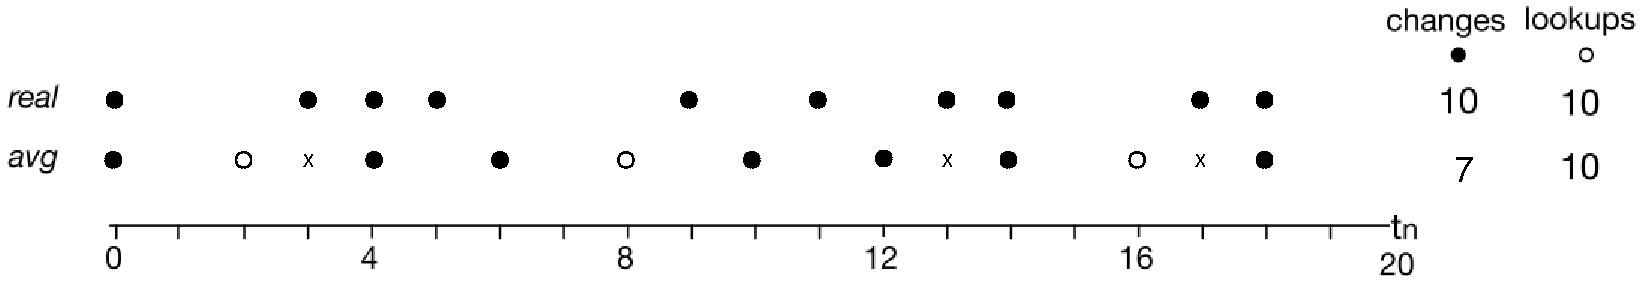
\includegraphics[width=1\linewidth]{syn.pdf}
	\caption{Change's history of a data and how average strategy capture or miss those changes.}
	\label{fig:syn}
\end{figure}

In this Section, we classify synchronization methods according to several dimensions characterizing their algorithms, such as (i) whether the synchronization is triggered by the consumer (pull-based) or the source (push-based), (ii) the ability to deterministically recognize the update time, and (iii) the foundation of estimation methods. Based on this classification, we review the methods proposed in the literature to solve the updating problem. Additionally, we compare the surveyed methods with respect to other dimensions, such as resource constraints they consider during the update process, quality achieved, datasets used, and dynamic features they consider.

\subsection{Synchronization Policies}\label{Synchronization}
~\cite{UmbrichHHPD10}

There are two possibilities to collect the change time for a given resource:
\begin{itemize}
	\item push-based approaches for which the data publishers provide change notifications.
	\item pull-based approaches for which one periodically checks if a data source has changed.
\end{itemize}

The push-based approach ensures that updates are reported to clients in a timely manner and is useful for many applications. However, push-based delivery may not be cost effective or feasible in all situations. Some scenarios are well suited to push, for example, a small group of clients who need to be notified of updates in a timely manner. In this case, push-based strategies could eliminate the need for clients to frequently poll servers, thereby reducing server load. However, only data providers can offer an information service based on push and it is not available in most cases. Therefore, applications have to rely on the other, pull-based approach, to collect change information. 

The pull-based monitoring approach has the obvious drawbacks of being more resource consuming than push-based change information. In addition, the monitoring interval influences how accurately one can sample the change times. For instance, the monitoring approach can only detect the last change between two monitoring intervals, even if several changes occurred during two monitoring points.

Table~\ref{tab:syn} lists some work that has been proposed for communication between dataset consumers and publishers.

% Table generated by Excel2LaTeX from sheet 'Hoja2'
\begin{table}[htbp]
	\centering
	\caption{Summary of synchronization mechanism.}
	\begin{tabular}{lcc}
		\hline
		Mechanism & Push & Pull \\ \hline
		SparqlPuSH \cite{PassantM10} & \cmark   & \\
		DSNotify \cite{PopitschH11} &   & \cmark \\
		online services\footnotemark & \cmark   & \\
		PubSubHubbub \cite{Fitzpatrick10} & \cmark   & \\
		Semantic Pingback \cite{TrampFEA10} & \cmark   & \\
		RDFSync \cite{TummarelloMBE07} &   &  \cmark  \\
		rsine \cite{MaderMS14} & \cmark   & \\
		Boca RDF \cite{MissierACDG07} & \cmark   & \\
		Atom \cite{Nottingham05} &    &  \cmark \\
		\hline
	\end{tabular}%
	\label{tab:syn}%
\end{table}%

\footnotetext{http://www.changedetection.com/}

\subsubsection{Change Notifications}\label{Notifications}
~\cite{UmbrichVH10}
Ideally, the consumer wants to be informed about the statements that have been added/removed at a certain time point. The notification about changes offers an efficient way to keep their data updated.

The study of Linked Data notifications is very relevant for a broad range of application domains. Currently, one of the most popular Linked Data notification approach, sparqlPuSH~\cite{PassantM10}, allows users to register a SPARQL query and get updates pushed to the user as new matching triples arrive in an underlying triple store containing relevant data. It relies on SPARQL queries, tracks changes of the result set published as an RSS feed, and broadcasts change notifications via the PubSubHubbub protocol. A more recent work is Resource Subscription and Notification sErvice (rsine)~\cite{MaderMS14}, a framework that notifies subscribers whenever resources are updated, created, or removed. It is comparable to sparqlPuSH, but it is designed to operate on a more general level, not only queries. In contrast to sparqlPuSH, rsine intends to maintain the quality of controlled vocabularies. Boca RDF~\cite{MissierACDG07} provides a change detection sub-system based on Sun’s Java messaging service. Users will get notifications when there is any change in individual RDF statements or the entire graph.

The push scenario assumes that the data provider sends the change notification to the client or to a hub, therefore, the change history will contain the complete set of all change times. While, push-based mechanisms can deal very efficiently with data that changes frequently, on the other hand, these mechanisms must maintain a subscriber list and open connection states that can also cause scalability problems as the number of clients grows. On the other hand, pull-based mechanisms consume more bandwidth resources.\\

\subsubsection{Change Monitoring}\label{Monitoring}
~\cite{UmbrichHHPD10}

%HTTP-metadata Monitoring

Given that the HTTP protocol is recommended by the Linked Data guidelines, the most intuitive way for clients to detect changes would be to exploit the HTTP header information provided on the Web.

The information contained in HTTP response headers offers fields to indicate a change in a document. Using such methods of change detection is more economical in that it avoids the need for content sniffing, but some works~\cite{UmbrichHHPD10, DividinoKG14, Kjernsmo15, NeumaierU16} show that these data are often not provided or are wrong.

Dividino et al.~\cite{DividinoKG14} evaluated the conformance of LOD data source to provide a valid and correct $Last$-$Modified$ HTTP header field, which indicates the date and time at which the resource was last modified. Their experiment shows that overall and on average only 8\% of the resources in the datasets provide correct values for this field. This number is far too low to be of use for any practical application.

Umbrich et al.~\cite{UmbrichHHPD10} verified the use (or lack of) of the $Etag$ and $Last$-$Modified$ field for a corpus of 550K documents and found that 67.95\% did not report either of these two fields. Therefore, it is not feasible to rely on this information to detect changes.

Kjernsmo~\cite{Kjernsmo15} investigated many of the HTTP caching implementations (i.e., LOD servers) and examines the availability and conformance of the HTTP headers that may allow caching. Even on different datasets, the authors conclude that the headers do not reflect the standards compliant lifetimes advertised by servers, and therefore they are not helpful for applications relying on caching.

Neumaier and Umbrich~\cite{NeumaierU16} inspected the HTTP Headers of a total of 3.1 million resources reveals that 66\% of the CKAN, 100\% of the Socrata and 0\% of the OpenDataSoft resources have the $Last$-$Modified$ header field.

To investigate the use of temporal information, Rula et al. ~\cite{RulaPHSM12} ascertained how many of the URIs that identified documents in the 2011 Billion Triple Challenge (BTC) dataset returned date information in the HTTP header. For that, they generated a random sample of 1000 documents (from the context of the quads), and for each document URI in the sample and they perform an HTTP lookup to check the $Last$-$Modified$ header in the HTTP response. They found again that only 95 out of 1000 URIs returned $Last$-$Modified$ headers.  

The Sitemap extension~\cite{CyganiakSDDT08} offers another solution, defining how often data can be re-crawled from a website to get fresh information, but it relies on clients regularly fetching it, not directly solving the synchronization issue. 

\subsubsection{Change Prediction}\label{Prediction}
~\cite{UmbrichHHPD10,BarsottiDD17a,GonzalezH18}

Typically, dataset providers do not offer any mechanism to inform clients about data updates: if the data has changed nor to what extent. Therefore, in this Section, we focus on synchronization strategies that are dataset agnostic, i.e., strategies that do not assume meta-data about what has changed since the last update. Table~\ref{tab:pull} shows surveyed works relating to Pull-Based Synchronization Approaches.\\

\begin{table*}[h]
	\centering
	\caption{Overview of Pull-Based Synchronization Approaches.}
	\label{tab:pull}
	\begin{tabular}{llll} \hline
		Works                                            & Year & Models                          & Datasets          \\ \hline
		Umbrich et al. \cite{UmbrichHHPD10}                & 2010 & Poisson Process                          & MultiCrawler        \\
		Umbrich et al. \cite{UmbrichMP15}                 & 2015 & Adaptive Heuristics, Markov Chains           & Wikipedia          \\
		Dividino et al. \cite{DividinoGS15}                & 2015 & History Metrics     & DyLDO            \\
		Neumaier and Umbrich \cite{NeumaierU16}         & 2016 & Empirical Distribution, Poisson Process, Markov Chains              & CKAN, Socrata, OpenDataSoft \\
		Knuth et al. \cite{KnuthHS16}                   & 2016 & History Metrics, Adaptive Heuristics & DBpedia Live         \\
		Nishioka and Scherp \cite{NishiokaS17}          & 2017 & Machine Learning     & DyLDO            \\
		Akhtar et al. \cite{AkhtarAL17}                  & 2017 & History Metrics                  & DyLDO(DBpedia), LSQ     \\
		Gonz\'{a}lez and Hogan \cite{GonzalezH18}         & 2018 & Machine Learning                         & Wikidata  \\  \hline      
	\end{tabular}
\end{table*}

\textbf{Empirical Distribution}: 

A simple method is to build an Empirical Distribution function based on the intervals between observed changes. An Empirical Distribution function is a distribution function associated with the empirical measure of a sample. This cumulative distribution function is a step function that jumps up by $ \frac{1}{n} $ at each of the $ n $ data points. Its value at any specified index of the measured variable is the fraction of observations of the measured variable that are less than or equal to that at the specified index.

\begin{example}
	\label{ex:ED}
	Based on the following change history (00111000100011000100001), where 0 indicates no change, and 1 a change based on comparing the content at the current point with the content at the previous sampling point. This history results in the intervals (31144145) which one can use as input for an Empirical Distribution.
\end{example}

Neumaier and Umbrich~\cite{NeumaierU16} evaluated this method for estimating freshness in Open Data Portals.\\

\textbf{Poisson Process}:

Cho and Garcia-Molina~\cite{ChoG00} modeled change frequencies of Web documents as Poisson Processes. The Poisson Process is one of the most widely-used counting processes. It is usually used in scenarios where we are counting the occurrences of certain events that appear to happen at a certain rate, but completely at random. For instance, occurrences of fatal auto accidents, arrivals of customers at a service center, telephone calls originating in a region, etc., are usually modeled by a Poisson Process. 

It is believed that a Poisson Process is a good model for changes on the Web of Data too. However, we found no studies showing that the assumption of a Poisson Process also holds for the sources on the Web of Data.

To describe the Poisson-process model, we use $X(t)$ to refer to the number of occurrences of a change in the interval $(0, t]$. Then, a Poisson Process of $rate$ or $frequency$ $\lambda$ has the following property:

For $s \geq 0$ and $t > 0$, the random variable $X(s + t) - X(s)$ has the Poisson probability distribution

\begin{equation}
\label{eq:Poisson}
P\\(X(s + t) - X(s) = k\\) = \frac{(\lambda t)^k}{k!}e^{-\lambda t} for~k=0,1,...
\end{equation}

Umbrich et al.~\cite{UmbrichHHPD10} analyzed whether they can apply this Poisson model to the changes of documents and entities detected on LOD and concluded they cannot accept nor reject the described change model with statistical significance.

Neumaier and Umbrich~\cite{NeumaierU16} followed an improved estimator provided by Cho and Garcia-Molina~\cite{ChoG03} to avoid the effects of incomplete change history. They improved this estimator, because they showed that the estimation is highly biased if the update history is incomplete, i.e., if there are changes to the resource, which are not detected by the sampling. However, in the case of this work, the results were not notably different from those of the traditional Poisson Process.\\

\textbf{Markov Chains}:

Another strategy is to apply the Markov Chains approach to determine the likelihood to observe a change in future considering the past observed changes. 

A Markov chain is a probabilistic process where the probability distribution of the next state depends on the current state only. This is stated in the so-called Markov property: given a present state, the future and past states are independent.

\begin{example}
	Using the change history of Example~\ref{ex:ED}, we can build a state-change matrix by counting the state transitions. Figure~\ref{tab:state1} shows the example considering only the last state of the data to compute the likelihood of the next state. For instance, the value (i = 1, i + 1 = 1) indicates that we observed 3 times that the data changes consecutively in a row and that we observed 5 times a change after a non-change (i = 0, i + 1 = 1). We use this information to determine how likely it is that the data changes in the next time: For instance, considering our example table: $P(1|0) = \frac{5}{15} = 0.33$. Figure~\ref{tab:state2} considers the last two change states of the data to compute the likelihood of the next change state.
\end{example}    

\begin{figure}[h]
	\begin{minipage}[b]{0.45\linewidth}
		\begin{tabular}{c|rr|c}
			i\textbackslash{}i+1 & 0  & 1 & TOTAL \\    \hline 
			0                    & 10 & 5 & 15    \\
			1                    & 4  & 3 & 7     
		\end{tabular}
		\caption{State-change matrix with depth 1.}
		\label{tab:state1}
	\end{minipage}
	\hspace{0.5cm}
	\begin{minipage}[b]{0.45\linewidth}
		\centering
		\begin{tabular}{c|rr|c}
			i-1;i\textbackslash{}i+1 & 0 & 1 & TOTAL \\    \hline 
			0;0                    & 5 & 5 & 10    \\
			0;1                    & 2 & 2 & 4     \\
			1;0                    & 4 & 0 & 4     \\
			1;1                    & 2 & 1 & 3    
		\end{tabular}
		\centering
		\caption{State-change matrix with depth 2.}
		\label{tab:state2}
	\end{minipage}
\end{figure}

Umbrich et al.~\cite{UmbrichMP15} used Markov Chains to schedule the next crawl time for URLs based on previously observed changes to the content. They used two variations of the Markov models considering only the last state and the last two change states of a document to compute the likelihood of change in the next state and they indicated that this strategy based on state-change transitions probabilities provide promising results.

Neumaier and Umbrich~\cite{NeumaierU16} examined and evaluated different freshness estimation heuristics, in particular, heuristics implemented and evaluated based on Empirical, Poisson, and Markov processes using several parameters with the purpose of estimating freshness in Open Data Portals.\\

\textbf{Adaptive Heuristics}:

Another strategy is to capture the Time-To-Live (TTL) of the dynamic data in an adaptive way. TTL determines specific time points when the data should be updated. To this end, each data item is associated with a value indicating a time interval after which the data needs to be updated. After the update, it is decided to increase or decrease the value based on observed changes. It is common to fix a minimum and maximum value.

The TTL mechanism leads to an interesting trade-off between the stale data traffic ratio and the redundant data update cost. In general, large TTL values lead to more stale data while small TTL values lead to higher processing overhead.

Depending on how one decides the value after the evaluation, there are many variations. If the data has changed, in general, the TTL value will be reduced, while if the data remains the same, the TTL will be increased. To determine the new value an increment function $F(.)$ is used. The function $F(.)$ takes as input the current TTL value $T^\prime$ of the data and outputs an increment value $F(T^\prime)$ to be added to the current TTL value, i.e., the new TTL value $ T $ is computed by the formula $T=T^\prime+F(T^\prime)$.

Alici et al.~\cite{AliciAOCU12} studied the problem of establishing adaptive TTL for query result caching in Web Search Engines and summarized the most used increment functions (see Table~\ref{tab:funtion}).

\begin{table}[h]
	\centering
	\caption{Increment functions.}
	\label{tab:funtion}
	\begin{tabular}{lll} \hline 
		Type        & $F(.)$ & Parameter \\    \hline \\
		Linear      & $c \times T^\prime$      & $\frac{1}{10}$, $\frac{1}{5}$, $\frac{1}{2}$     \\ \\
		Polynomial  & $(T^\prime)^c$      & $ -3 $, $ -2 $, $ -1 $, $-\frac{1}{2}$, $\frac{1}{2}$   \\	\\
		Exponential & $c^{T^\prime}$      & $\frac{1}{2}$, $ 1 $, $ 2 $    \\  \\  \hline     
	\end{tabular}    
\end{table}

Umbrich et al.~\cite{UmbrichMP15} introduced and evaluated three adaptive strategies in terms of accurately capturing the changes of data and also estimated the crawl time for a given set of URLs with the aim of optimally scheduling the refresh of URLs with limited resources.

Knuth et al.~\cite{KnuthHS16} investigated multiple performance metrics of scheduling strategies for the re-execution of queries on a dynamic dataset. They evaluated a simple incremental method to estimate the Time-to-Live (TTL) of queries.\\

\textbf{History Metrics}:

Another strategy is to explore different characteristics extracted from execution history to assign a score of importance to each data item and, thus, derive an update order.

A programming strategy aims to derive an order of importance for data elements based on a set of data characteristics. In the ideal case, a strategy would derive an order such that the application would update only the subset of LOD sources that have actually changed.

It is possible to implemented different scheduling policies using the following features:
\begin{itemize}
	\item \textbf{Age} describes the actual time passed since the last item update.
	\item \textbf{Execution Time} describes how long it takes to update the item.
	\item \textbf{Change Rate} indicates “how often” an item has changed.
	\item \textbf{Change Dynamics} indicates “to what extent” an item has changed. It is an aggregation of changes over the previous item updates. We compute this metric by using the quantification metrics (distance) between known subsequent results.
	\item \textbf{Change Ratio} indicates the absolute number of changes of the data between the last two (known) observation points in time.
	\item \textbf{Size} indicates the size of items.
\end{itemize}

As a large number of items may have changed, but only a limited number can be updated per time, it is necessary to determine which items should be refreshed first. By using the vector of features of each item, we can define an update function $ \rho: f \rightarrow R$, which assigns a preference score to a data source based on the observed features at time $t_i$. An update strategy is defined by ranking the data according to their preference score in descending or ascending order and fetching them, starting from the top-ranked entry to some lower ranked entry. For instance, if we consider $size$ to be the feature observed at time $t_i$ for all items $c$, $\rho$ could be defined as the rank of the size of items in ascending order (from the smallest to the biggest ones).

These techniques under unbounded resources obtain maximum accuracy executing complete updates every time. Therefore, to compare different proposals it is necessary to evaluate them under the same restrictions and data. Some works have been developed~\cite{DividinoGS15, KnuthHS16, AkhtarAL17} to evaluate the quality of these strategies in different scenarios.\\

\textbf{Machine Learning}:

Aligned with the previous approaches, we can try to predict future changes using methods from Data Mining and Machine Learning. With an ML model, we can learn what classes of dynamics can and should we distinguish or what features should these methods be based on.

In general, we can model this problem in different ways, such as a linear regression problem, if we want to predict the TTL of the data or as a binary classification problem, if we want to predict if the data will change in the next time interval.

The characteristics depend on the object to be studied, although it would be useful to capture the tendency of the data to change. Also, one can study how effective are the features to estimate changes. The expectation is that the number of changes will provide clues about the freshness period.

Nishioka and Scherp~\cite{NishiokaS17} computed a Linear Regression Model in order to identify features that have a large influence on the lifespan of the triples. 

Gonz\'{a}lez and Hogan~\cite{GonzalezH18} used a Linear Regression Model to predict the future distribution of concepts modeled based on a lattice of Characteristic Sets. 

\subsection{Scheduling Strategies}\label{Scheduling}
~\cite{AkhtarAL17}

\subsection{System Summary}\label{System2}
\subsection{Summary}\label{Summary2}
\subsection{Open Questions}\label{Open2}

\section{Query Analysis}\label{Query}
\subsection{Query Dynamics}\label{Dynamics}
\subsection{Query Caching}\label{Caching}


\subsection{Continuous Query Processing}\label{Streams}

~\cite{DehghanzadehDGV15}

\subsection{Linked Data Fragments}\label{Fragments}
\subsection{System Summary}\label{System4}
\subsection{Summary}\label{Summary4}
\subsection{Open Questions}\label{Open4}











%\begin{figure}[t]
%\includegraphics{}
%\caption{Figure caption.}\label{f1}
%\end{figure}

%\begin{table*}
%\caption{} \label{t1}
%\begin{tabular}{lll}
%\hline
%&&\\
%&&\\
%\hline
%\end{tabular}
%\end{table*}

%%%%%%%%%%% The bibliography starts:

%%%%%%%%%%%%%%%%%%%%%%%%%%%%%%%%%%%%%%%%%%%%%%%%%%%%%%%%%%%%%
%%                  The Bibliography                       %%
%%                                                         %%
%%  ios1.bst will be used to                               %%
%%  create a .BBL file for submission.                     %%
%%                                                         %%
%%                                                         %%
%%  Note that the displayed Bibliography will not          %%
%%  necessarily be rendered by Latex exactly as specified  %%
%%  in the online Instructions for Authors.                %%
%%                                                         %%
%%%%%%%%%%%%%%%%%%%%%%%%%%%%%%%%%%%%%%%%%%%%%%%%%%%%%%%%%%%%%

\newpage
\nocite{*} 
% if your bibliography is in bibtex format, use those commands:
\bibliographystyle{ios1}           % Style BST file.
\bibliography{bibliography}        % Bibliography file (usually '*.bib')

% or include bibliography directly:
%\begin{thebibliography}{0}
%\bibitem{r1} F. Author, Information about cited object.
%
%\bibitem{r2} S. Author and T. Author, Information about cited object.
%\end{thebibliography}

\end{document}
